En esta seccion vamos a realizar una conclusi\'on general de los distintos algoritmos. En base a la performance de los mismos y las distancias con respecto a la soluci\'on Exacta.

Primero planteamos un experimento en el cual corrimos para instancias aleatoreas, nuevamente con las tres densidades utilizadas a lo largo de todo el Trabajo Pr\'actico(15\%, 50\% y 100\%), todos los algoritmos (Exacto con podas, Heuristica Golosa, Heuristica de Busqueda Local y Heuristica GRASP) unas 50 veces para cada cantidad de nodos entre 5 y 20 (por ser numeros manejables para el algoritmo exacto) para sacar un promedio de cuanto difiere cada Heuristica contra el algoritmo Exacto.\\
Para esto calculamos la peor soluci\'on para cada instancia (que ser\'ia ubicar todos los nodos en una \'unica partici\'on, con lo cual la sumatoria de las aristas intrapartici\'on ser\'a la sumatoria total de las aristas) y generamos una formula que nos representa un valor entre 1 y 0 que tanto diverge la Heuristica en relaci\'on al exacto, pero considerando el valor entre la peor soluci\'on y la soluci\'on ideal.
La formula es: 

\bc
1 - ((solucionHeuristica - solucionExacto)/(peorSolucion - solucionExacto))
\ec

Si la Heuristica tiene el mismo valor que el Exacto esta relaci\'on nos devuelve que es 1. Todo lo contrario si la heuristica devuelve la peor soluci\'on, esta formula nos retorna 0.\\
Con lo cual es un buen indicador para saber cuan buena es la soluci\'on de una de las heuristicas.

\subsection{Divergencia de las Heuristicas}

\subsubsection{2 Particiones}

\begin{figure}[H]
\begin{center}
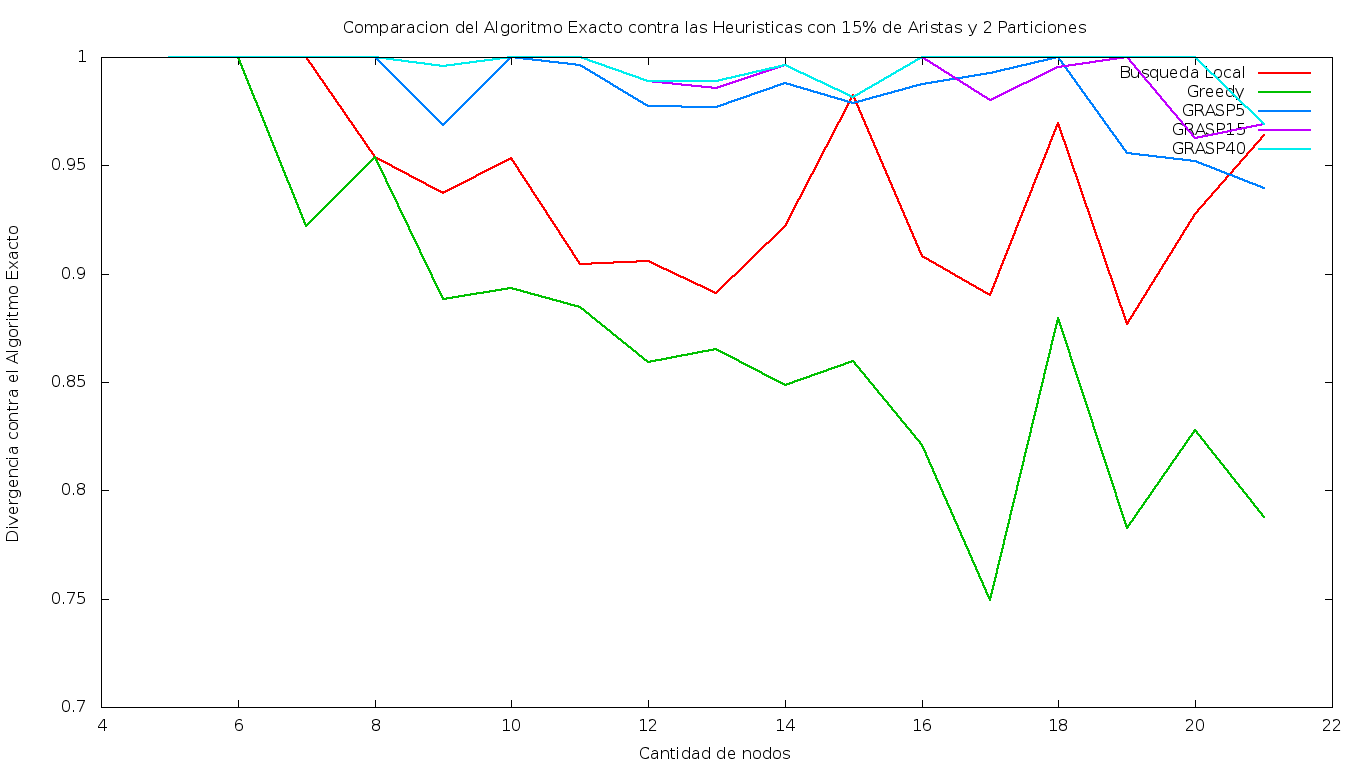
\includegraphics[scale=0.3]{finales/ComparacionesCon2Particiones15Aristas.png}
\caption{Distancias de las Heuristicas para K = 2 y 15\% de aristas}
\end{center}
\end{figure}

\begin{figure}[H]
\begin{center}
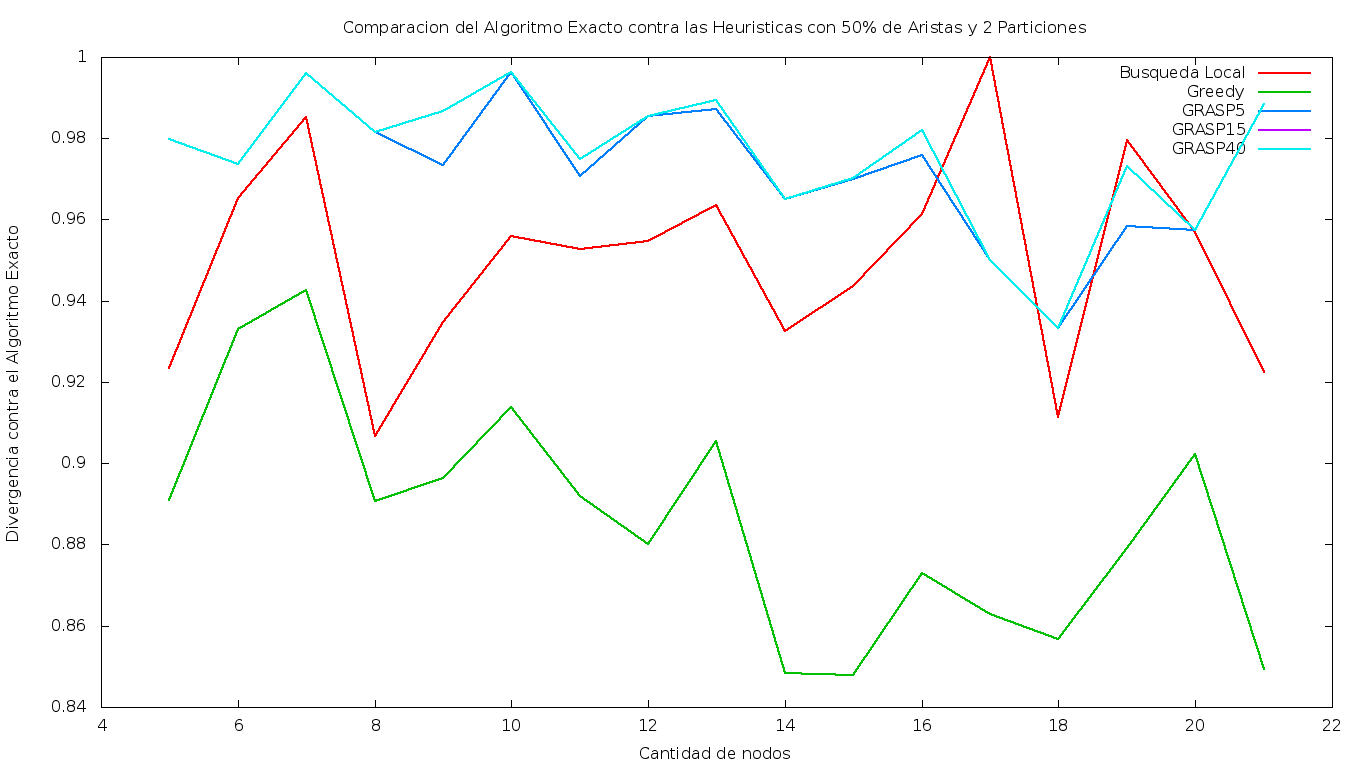
\includegraphics[scale=0.3]{finales/ComparacionesCon2Particiones50Aristas.png}
\caption{Distancias de las Heuristicas para K = 2 y 50\% de aristas}
\end{center}
\end{figure}

\begin{figure}[H]
\begin{center}
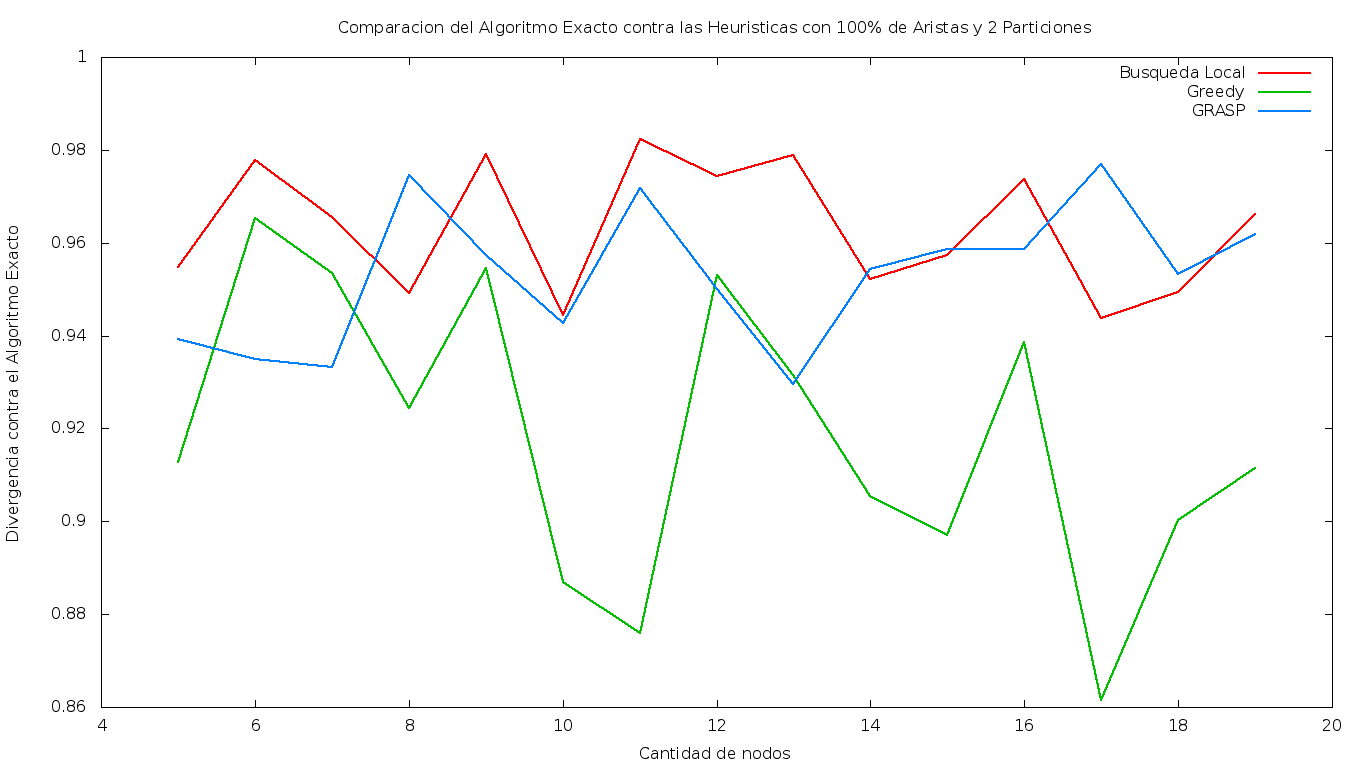
\includegraphics[scale=0.3]{finales/ComparacionesCon2Particiones100Aristas.png}
\caption{Distancias de las Heuristicas para K = 2 y 100\% de aristas}
\end{center}
\end{figure}



Podemos ver como a medida que aumenta la cantida de nodos los valores de divergencia de las Heuristicas comienzan a aumentar.

Otro punto f\'acilmente apreciable es que la Heur\'istica Greedy es'